\documentclass[11pt]{scrartcl}
%\documentclass[11pt,twoside]{article}

%opening
\newcommand{\lecid}{15-316}
\newcommand{\course}{Software Foundations of Security and Privacy}
\newcommand{\lecdate}{} %e.g. {October 21, 2013}
\newcommand{\lecnum}{10}
\newcommand{\lectitle}{Security Automata}
\newcommand{\lecturer}{Matt Fredrikson}
\newcommand{\lecurl}{https://15316-cmu.github.io/index}

\usepackage{varwidth}
\usepackage{lecnotes}
\usepackage[irlabel]{bugcatch}

\usepackage{tikz}
\usetikzlibrary{automata,shapes,positioning,matrix,shapes.callouts,decorations.text,patterns,trees,backgrounds}

% \usepackage[bracketinterpret,seqinfers,sidenotecalculus]{logic}
% \newcommand{\I}{\interpretation[const=I]}

% \newcommand{\bebecomes}{\mathrel{::=}}
% \newcommand{\alternative}{~|~}
% \newcommand{\asfml}{F}
% \newcommand{\bsfml}{G}
% \newcommand{\cusfml}{C}
% \def\leftrule{L}%
% \def\rightrule{R}%

\begin{document}

\newcommand{\atrace}{\sigma}%
%% the standard interpretation naming conventions
\newcommand{\stdI}{\dTLint[state=\omega]}%
\newcommand{\Ip}{\dTLint[trace=\atrace]}%
\newcommand{\ws}{\omega}\newcommand{\wt}{\nu}% 

\maketitle
% \thispagestyle{empty}

%%%%%%%%%%%%%%%%%%%%%%%%%%%%%%%%%%%%%%%%%%%%%%

\section{Introduction \& Recap}

We began studying safety properties by intuiting that they describe systems where something ``bad'' never happens, and have seen that contracts, assertions, memory safety, and more granular forms of sandboxing are all instances of safety.
But there are certainly other types of bad events that we might want to write policies to enforce against, and aside from finding a way to encode them in programs using assertions, it isn't clear how we would go about doing this.

In Lecture 8 we developed symbolic evaluation, an algorithmic proof procedure for dynamic logic judgments about programs. Symbolic evaluation works with sequents of the form
\[
  \Gamma \Vdash S
\]
where $\Gamma$ is a set of pure assumptions (path constraints) and $S$ is a stack built from pure formulas and box modalities (e.g., $Q$ or $[\alpha]S$). The proof rules mirror evaluation order: composition pushes a continuation onto the stack, assignments introduce fresh variables/equalities, and conditionals split into branches while extending $\Gamma$. When the succedent is pure, we discharge the goal using an arithmetic oracle.

One useful way to read symbolic evaluation is as a symbolic execution tree. Each branch corresponds to a family of concrete executions, and the evolving assumptions $\Gamma$ describe the concrete program states that can arise along that branch.

Today we shift from proving properties about programs to enforcing policies by monitoring a program as it executes. A runtime monitor observes the program's execution trace (states, events, or other chosen observations), maintains its own internal state, and intervenes when it detects that execution is about to violate a policy.

This raises a fundamental question: which policies can be enforced by watching a program execute and intervening based only on what we have observed so far? In this lecture we study how to characterize this enforceable class and how to represent such policies using security automata~\cite{Schneider2000}, small state machines that read the observed trace and reject as soon as a bad prefix appears.
\section{Security automata}

When a program runs, it produces an observable \emph{trace} that we can think of as a sequence
\[
\sigma = \sigma_0,\sigma_1,\ldots
\]
of ``steps'' of execution. In the most concrete view, a step might be the entire program state $\omega$ (a valuation of variables, memory, etc.). But for many policies we instead view each step as an \emph{event}: a system call, an API invocation, a message received over the network, and so on. The point is that a safety policy rules out certain \emph{bad prefixes} of this trace.

A \emph{security automaton} is a convenient way to represent and enforce such policies: the automaton's state summarizes the relevant history of the trace so far, and each transition is guarded by a predicate describing which next steps are allowed. We will use the convention that we draw only the transitions that keep the policy satisfied; if no transition is enabled, the current prefix must be bad and the policy is violated.

\subsection{Runtime-enforceable trace properties}
At runtime, an enforcement mechanism only observes a growing \emph{prefix} of the trace and can react by intervening (e.g., aborting execution). This imposes some basic structure on the kinds of policies we can hope to enforce.
\begin{itemize}
\item \textbf{Trace condition.} A policy must be a condition on a program trace. That is, whether the policy holds should be determined only by the observed sequence $\sigma$ of states/events that execution produces, as opposed to requiring information about other executions that did not occur, or external factors that may not be accessible when the program executes.

\item \textbf{Prefix closure.} Once the policy is violated, later execution cannot ``repair'' it. Formally, if a prefix $\tau$ is already a violating prefix, then any extension of $\tau$ is also violating.

\item \textbf{Finite refutability.} Violations must have a finite witness: if a full trace violates the policy, then there exists a finite bad prefix after which all extensions still violate. This is exactly what makes runtime detection possible: a monitor only needs to watch until a bad prefix appears.
\end{itemize}
These are the hallmarks of \emph{safety} properties: ``nothing bad ever happens'' means that if something bad happens, we can point to the finite moment when it first did.

\subsection{Example: No \texttt{send} after \texttt{readfile}}
Suppose our trace consists of system-call instructions/events such as \pread (read from a local file) and \psend (send to the network). We want to enforce:
\begin{quote}
after a \texttt{readfile}, there must not be any subsequent \texttt{send}.
\end{quote}
Let $c$ denote the system call executed at the current step. The following security automaton enforces this policy.
\begin{center}
\scalebox{1.2}{%
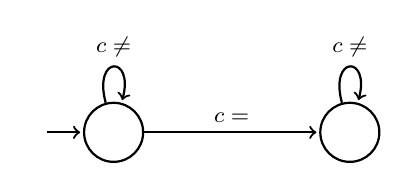
\begin{tikzpicture}
[
  highlight/.style={draw=blue, text=blue},
  shorten >=1pt,
  node distance=2cm,
  on grid,
  auto,
  /tikz/initial text={},
  font=\footnotesize,
  thick
]
 \node[state,thick,initial left,inner sep=1pt,minimum size=0.75cm] (l0) {};
 \node[state,thick,inner sep=1pt,minimum size=0.75cm] (l1) [right=3cm of l0] {};

  \path[->] 
    (l0) edge [thick,loop above] node [above] {$c \ne \pread$} (l0)
    (l0) edge [thick] node [above] {$c = \pread$} (l1)
    (l1) edge [thick,loop above] node [above] {$c \ne \psend$} (l1);
\end{tikzpicture}
	}
	\end{center}
	There are no accepting states in a security automaton: as long as there is some enabled transition from the current policy state, the policy has not been violated. Here, once we have seen a \pread event, we move to the rightmost state, where only events satisfying $c \ne \psend$ are permitted. If the program executes \psend at that point, there is no transition to take and the monitor concludes that the prefix is bad.

Sometimes we care about both which event occurred and some property of the program state at that moment. One simple way to model this is to let the input symbol include both pieces of information (e.g., $\sigma_i$ could be a pair consisting of the current state and the current event), and then write transition guards that mention both.

For example, we might relax the previous policy to allow a \psend after \pread only if a program variable $\mathit{ok}$ indicates the data has been sanitized. 
When $\mathit{ok}=1$ the implication is trivially true (so \psend is permitted), and when $\mathit{ok}\ne 1$ it reduces to $c \ne \psend$.
\begin{center}
\scalebox{1.2}{%
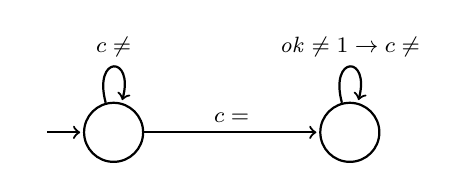
\begin{tikzpicture}
[
  highlight/.style={draw=blue, text=blue},
  shorten >=1pt,
  node distance=2cm,
  on grid,
  auto,
  /tikz/initial text={},
  font=\footnotesize,
  thick
]
 \node[state,thick,initial left,inner sep=1pt,minimum size=0.75cm] (l0) {};
 \node[state,thick,inner sep=1pt,minimum size=0.75cm] (l1) [right=3cm of l0] {};

  \path[->]
    (l0) edge [thick,loop above] node [above] {$c \ne \pread$} (l0)
    (l0) edge [thick] node [above] {$c = \pread$} (l1)
    (l1) edge [thick,loop above] node [above] {$\mathit{ok} \ne 1 \rightarrow c \ne \psend$} (l1);
\end{tikzpicture}
}
\end{center}
If the program attempts to execute \psend when $\mathit{ok}\ne 1$, then the guard is false and there is no enabled transition, so the policy is violated.

\subsection{Definition}
Next we define security automata and what it means for them to accept traces.

\begin{definition}[Security automaton\cite{Schneider2000}]
\label{def:sa}
A security automaton is a nondeterministic state machine that consists of the following components:
\begin{itemize}
\item a countable set $O$ of automaton states,
\item a countable set $O_0 \subseteq O$ of initial states,
\item a countable set $\Sigma$ of transition symbols (the alphabet of observable steps/events in traces $\sigma$),
\item a transition relation $\delta \subseteq O \times \powerset{\Sigma} \times O$ between automaton states and sets of transition symbols.
\end{itemize}
\end{definition}

We will assume that sets of transition symbols are represented by formulas (predicates) that can be evaluated over input symbols (events).
Concretely, the set of symbols corresponding to a formula is comprised of exactly the symbols that the formula is true of.
Given a sequence of transition symbols (events) $\sigma = \sigma_0,\sigma_1,\ldots$, we say that the automaton accepts $\sigma$ if and only if there is a corresponding sequence of states $o = o_0,o_1,\ldots$ such that for each pair $\sigma_{i},\sigma_{i+1}$ in $\sigma$,
\begin{itemize}
\item there is a corresponding pair $o_{i},o_{i+1}$ of states in $o$,
\item and there exists $(o_{i}, P, o_{i+1}) \in \delta$ where $\sigma_i \vDash P$.
\end{itemize}
In other words, a trace is only accepted if there is a corresponding run of the automaton that always follows the transition function.

The choice of transition symbols $\Sigma$ is a design decision: it defines what the monitor gets to observe. In some settings a symbol might be a system call event like \pread or \psend, as in our examples above. In others, a symbol might be a full program state, or a structured observation such as a pair consisting of an event together with a snapshot of selected state. The key requirement is that the symbol stream contains enough information to recognize bad prefixes of the safety policy.

\subsection{Taint analysis}

We have seen that information flow cannot be checked by examining single traces in isolation. But this doesn't mean that they can't be \emph{approximated} in some useful sense by safety properties. One approach for approximating information flow that has been used widely for certain applications is called \emph{taint analysis}~\cite{Schwartz2010}. 

Conceptually, taint analysis enforces a safety property that tracks the portions of program state that have been ``tainted'' by some identified source. The policy maintains state that contains a bit for each variable and memory cell used by the target program. A subset of the variables and memory cells are distinguished as taint ``sources'', and a different subset as the ``sinks''. Then as the program executes, the policy state is updated to reflect the flow of tainted information through the state. If any of the state identified as a sink becomes tainted, then the policy is violated.

\paragraph{Security automaton.}
Taint analysis can be formalized and enforced as a security automaton. We show how by defining the states, initial states, transition symbols, and transition relation. To keep things simple while illustrating the main ideas, we will assume that the language has only variables and no memory state or operations.
\begin{itemize}
\item The states of the automaton correspond to the set of all \emph{taint mappings} $\taint$ from program variables to $\{0,1\}$. Intuitively, if the policy is in a state where $\taint(x) = 1$, then $x$ is currently tainted, and if $\taint(x) = 0$ then it is not.

\item The initial states are all mappings $T$ where $T(x) = 1$ for each identified source variable and $T(y) = 0$ for all non-source variables.

\item The transition symbols are program instructions $\pupdate{\pumod{x}{\astrm}}$, $\passert{\ivr}$, $\pifjump{\ivr}{\astrm}$.

\item The transition relation is defined to \emph{propagate} the taintedness of an expression on the right-hand side of an assignment to the variable on its left-hand side. If $\taint$ is a taint mapping, then we use the following rules to determine whether an expression is tainted.
\begin{center}
\begin{calculus}
\cinferenceRule[var|Var]{Var}{%
\linferenceRule[sequent]
  {\taint(x) = 1}
  {\lsequent{\taint}{x}}
}{}%
\end{calculus}
\quad
\begin{calculus}
\cinferenceRule[opl|OpL]{OpL}{%
\linferenceRule[sequent]
  {\lsequent{\taint}{\astrm}}
  {\lsequent{\taint}{\astrm \cdot \bstrm}}
}{}%
\end{calculus}
\quad
\begin{calculus}
\cinferenceRule[opl|OpR]{OpR}{%
\linferenceRule[sequent]
  {\lsequent{\taint}{\bstrm}}
  {\lsequent{\taint}{\astrm \cdot \bstrm}}
}{}%
\end{calculus}
\end{center}
Then for every assignment instruction $\pumod{x}{\astrm}$ where $x$ is not a sink variable, and pair of states $\taint_1, \taint_2$ where $\lsequent{\taint_1}{\astrm}$ and $\taint_2(x) = 1$, the corresponding edge $(\taint_1, \pumod{x}{\astrm}, \taint_2)$ is in the transition relation. Additionally, for every pair of states $\taint_1, \taint_2$ where $\taint_1 \not\vdash \astrm$ and $\taint_2(x) = 0$, $(\taint_1, \pumod{x}{\astrm}, \taint_2)$ is in the relation. Finally, for every other instruction $\asprg$ that is not an assignment and every state $\taint$, $(\taint, \asprg, \taint)$ is in the transition relation.
\end{itemize}
Let's see how this works for a simple program with variables $x, y,$ and $z$. Suppose that $x$ is a taint source, and $z$ is the sink:
\begin{equation}
\begin{array}{ll}
\mathtt{1:} & z := 0 \\
\mathtt{2:} & y := x \\
\mathtt{3:} & z := y
\end{array}
\end{equation}
The automaton will have eight states, as there are $2^3 = 8$ mappings from the three variables to $\{0,1\}$. We will use a shorthand to denote states that gives the value of the mapping on each variable $x,y,z$ in order. So the initial state maps $x$ to 1, and $y,z$ to 0 and is denoted \verb'[100]'. 

We will only consider edges corresponding to instructions in the program, so the initial state has three possible outgoing edges. On executing either $z := 0$ or $z := y$, none of the taint state changes so we would remain in the initial state. On executing $y := x$ however, the mapping for $y$ changes to 1 because $\lsequent{\mathtt{[100]}}{x}$. So the automaton can transition to \verb'[110]'.
\begin{center}
\scalebox{1.2}{%
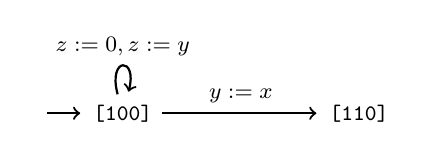
\begin{tikzpicture}
[
  highlight/.style={draw=blue, text=blue},
  shorten >=1pt,
  node distance=2cm,
  on grid,
  auto,
  /tikz/initial text={},
  font=\footnotesize,
  thick
]
 \node[rectangle,thick,initial left,draw=none] (l0) {\texttt{[100]}};
 \node[rectangle,thick,draw=none] (l1) [right=3cm of l0] {\texttt{[110]}};

  \path[->] 
    (l0) edge [thick,loop above] node [above] {$z := 0, z := y$} (l0)
    (l0) edge [thick] node [above] {$y := x$} (l1);
\end{tikzpicture}
}
\end{center}
From state \verb'[110]', executing $z := 0$ or $y := x$ leaves the taint mapping the same, but executing $z := y$ would result in \verb'[111]'. However, $z$ is a sink variable so entering this state would be a policy violation, and we leave the edge out.
\begin{center}
\scalebox{1.2}{%
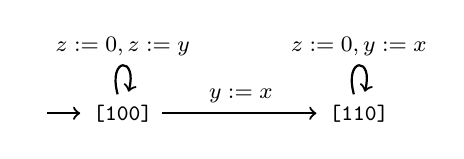
\begin{tikzpicture}
[
  highlight/.style={draw=blue, text=blue},
  shorten >=1pt,
  node distance=2cm,
  on grid,
  auto,
  /tikz/initial text={},
  font=\footnotesize,
  thick
]
 \node[rectangle,thick,initial left,draw=none] (l0) {\texttt{[100]}};
 \node[rectangle,thick,draw=none] (l1) [right=3cm of l0] {\texttt{[110]}};

  \path[->] 
    (l0) edge [thick,loop above] node [above] {$z := 0, z := y$} (l0)
    (l0) edge [thick] node [above] {$y := x$} (l1)
    (l1) edge [thick,loop above] node [above] {$z := 0, y := x$} (l1);
\end{tikzpicture}
}
\end{center}
The full automaton has additional states and transitions. For example, if the taint mapping were \verb'[010]', then executing $y := x$ would transition to \verb'[000]', whereas executing $z := 0$ would stay in the same state. Moreover, executing any instruction in \verb'[000]' stays in that state, so we would add this to the automaton.
\begin{center}
\scalebox{1.2}{%
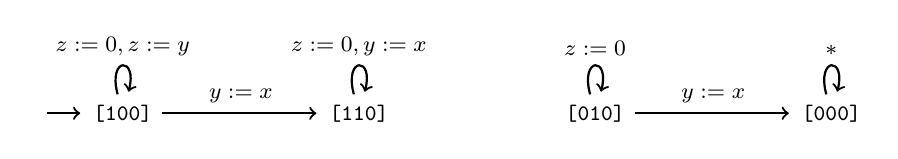
\begin{tikzpicture}
[
  highlight/.style={draw=blue, text=blue},
  shorten >=1pt,
  node distance=2cm,
  on grid,
  auto,
  /tikz/initial text={},
  font=\footnotesize,
  thick
]
 \node[rectangle,thick,initial left,draw=none] (l0) {\texttt{[100]}};
 \node[rectangle,thick,draw=none] (l1) [right=3cm of l0] {\texttt{[110]}};
 \node[rectangle,thick,draw=none] (l2) [right=3cm of l1] {\texttt{[010]}};
 \node[rectangle,thick,draw=none] (l3) [right=3cm of l2] {\texttt{[000]}};

  \path[->] 
    (l0) edge [thick,loop above] node [above] {$z := 0, z := y$} (l0)
    (l0) edge [thick] node [above] {$y := x$} (l1)
    (l1) edge [thick,loop above] node [above] {$z := 0, y := x$} (l1)
    (l2) edge [thick] node [above] {$y := x$} (l3)
    (l2) edge [thick,loop above] node [above] {$z := 0$} (l2)
    (l3) edge [thick,loop above] node [above] {$\mathtt{*}$} (l3);
\end{tikzpicture}
}
\end{center}
But these states are not reachable from the initial state of the SA, so we can leave them out and stop here.

\paragraph{Implicit flows.} So far taint analysis seems to do what we want in terms of tracking information flow as the program executes. So why did we say that it is an approximation of information flow, and moreover, why doesn't this contradict our thought experiment from earlier?

Recall that the program $\asprg_1$ in (\ref{eq:flowexp}) flowed information from $x$ to $y$, effectively computing $y = (1 - x)$. But it did not compute this using an assignment with $x$ on the right hand side, and rather with a conditional statement and constant assignments in either branch. This is known as an \emph{implicit flow} because the information moves from $x$ to $y$ indirectly by the choice of which program to execute within the conditional, rather than explicitly via an assignment statement.

The taint analysis policy that we described doesn't deal with implicit flows because it only propagates taintedness through explicit assignments. In this way taint analysis \emph{underapproximates} information flow. Whenever taint analysis deems that information has flowed from a source to a sink, then an information flow exists in the program. But if it fails to identify a flow, then we can't conclude that there isn't one in the program because there could yet be an implicit flow.

Can we change the security automaton policy to account for implicit flows? Suppose that we added an additional mapping to the policy state, intuitively corresponding to whether the program counter is tainted. We'll denote this $\taint(\pc)$, and we want to make sure that it is set to 1 whenever a conditional statement on a tainted expression is executed. So for example, if $x$ is a source in program (\ref{eq:implicit1}) below, then the policy will be in a state where $\taint(\pc)=1$ after executing the instruction at \keywordfont{1}.
\begin{equation}
\label{eq:implicit1}
\begin{array}{ll}
\mathtt{1:} & \pifjump{x \ne 0}{4} \\
\mathtt{2:} & y := 0 \\
\mathtt{3:} & \pifjump{\mathtt{true}}{5} \\
\mathtt{4:} & y := 1 \\
\mathtt{5:} & \ldots
\end{array}
\end{equation}
Then we can adapt the policy so that whenever $\taint(\pc) = 1$ in the current state, the target of \emph{any} assignment will become tainted. In (\ref{eq:implicit1}), this will ensure that $y$ is tainted after the conditional at \keywordfont{1}, and thus reflect the fact that there is an information flow from $x$ to $y$ in the program.

But now consider what happens if we add another instruction, as in (\ref{eq:implicit2}).
\begin{equation}
\label{eq:implicit2}
\begin{array}{ll}
\mathtt{1:} & \pifjump{x \ne 0}{3} \\
\mathtt{2:} & y := 0 \\
\mathtt{3:} & \pifjump{\mathtt{true}}{5} \\
\mathtt{4:} & y := 1 \\
\mathtt{5:} & z := 0
\end{array}
\end{equation}
Now under the current policy, $z$ will become tainted because it is executed after the tainted conditional. But there is clearly no flow of information from $x$ to $z$, so the taint mapping no longer reflects the actual flows in the program. Perhaps we could refine the policy further, by un-tainting the program counter once control returns to instructions that are in no way conditional on tainted data. In (\ref{eq:implicit2}), this is true for the assignment to $z$ at instruction \keywordfont{5} because it is executed regardless of the condition at \keywordfont{1}.

But how do we identify instructions that aren't conditional on tainted data in general? It was easy in this program, but things could get much more complicated as shown in (\ref{eq:implicit3}).
\begin{equation}
\label{eq:implicit3}
\begin{array}{ll}
\mathtt{1:} & \pifjump{x \ne 0}{6} \\
\mathtt{2:} & y := 0 \\
\mathtt{3:} & \pifjump{\precv\mathtt{()} \ne 0}{7} \\
\mathtt{4:} & \pifjump{\mathtt{true}}{6} \\
\mathtt{5:} & y := 1 \\
\mathtt{6:} & z := 0 \\
\mathtt{7:} & \ldots
\end{array}
\end{equation}
Now in order to tell whether to untaint the program counter before executing instruction 6, we need to predict the outcome of a network read. This policy has gotten significantly more complicated, and keep in mind that we need to do all of these calculations at runtime, which may impose considerable overhead on the target program.

Finally, even if we could solve this problem, tracking taint across implicit flows still may not accurately reflect a program's information flows. Consider the program in (\ref{eq:implicit4}) below.
\begin{equation}
\label{eq:implicit4}
\begin{array}{ll}
\mathtt{1:} & \pifjump{x \ne 0}{3} \\
\mathtt{2:} & y := 0 \\
\mathtt{3:} & \pifjump{\mathtt{true}}{5} \\
\mathtt{4:} & y := \mathtt{complicated\_function()} \\
\mathtt{5:} & \ldots
\end{array}
\end{equation}
It may turn out that $\mathtt{complicated\_function()}$ always returns 0, so that $y$ always takes the same value after the conditional regardless of what $x$ is. In this case, there is no real flow of information from $x$ to $y$. But our security automaton policy can't reason this way, because it would require considering a different trace from the one that was actually executed. Even if it could, it would need to reason about the behavior of an arbitrarily complicated, possibly non-terminating function, which is clearly not possible.

\subsection{Enforcing security automata policies}

The primary means of enforcing policies defined using security automata is with a reference monitor (RM). The RM is a mechanism that examines the program as it executes, using information about the current and past states to decide whether the policy has been violated. This is done according to Definition~\ref{def:sae}, and was sketched out at the beginning of this section.

\begin{definition}[Security automaton enforcement]
\label{def:sae}
Let $O_c$ be the current set of states that the security automaton is in. Then for each step that the program is about to take resulting in new program state $\omega$, the reference monitor does one of two things.
\begin{enumerate}
\item For each state $o \in O_c$ that the automaton can transition from, the states $\delta(o,P,o')$ for all transition edges where $\omega \vDash P$ are added to the new automaton states.
\item If the automaton cannot transition from any of its current states, then the program is not allowed to enter state $\omega$ and the reference monitor takes remedial action.
\end{enumerate}
\end{definition}

As long as the policy is not violated, then the RM allows the program to continue executing as it otherwise would. If the policy is violated, then the RM intervenes on the program execution to take some remedial action. This could mean simply aborting the execution, or something less drastic that prevents harm in other ways.

\paragraph{Necessary assumptions.} As pointed out by Schneider in his seminal work on security automata~\cite{Schneider2000}, there are several assumptions that one must make in order to enforce these policies effectively with a reference monitor. First, the reference monitor needs to simulate the execution of the automaton as the program runs, so it must keep track of which state the policy is in on the actual hardware running the program. This means that the automaton cannot require an unbounded amount of memory, so automata that have an infinite number of states are not in general enforceable.

Second, the RM must be able to prevent the program from entering a state that would result in a policy violation. This is called target control, and is a more subtle issue that it may at first seem. Take for example the policy of ``real-time'' availability, which states that a principal should not be denied a resource for more than $n$ real-time seconds. How could a reference monitor enforce this policy? It might try to predict the amount of time that it takes to remediate a trace that is about to violate the policy, and take action earlier than necessary to prevent the violation. But how does it know that the policy would have actually been violated in this case? Unless the reference monitor can literally stop time, this is not an enforceable policy.

Third, the program under enforcement must not be able to intervene directly on the state of the reference monitor. This is called enforcement mechanism integrity, and is crucial for ensuring that the policy defined by the automaton is the one that is actually enforced on the target program. We dealt with an instance of this issue earlier in the lecture, when we used control flow integrity to make sure that inlined safety checks weren't bypassed by indirect jumps. But now that the policy itself has state, the enforcement mechansim must also guarantee that the target program does not make changes to that state or influence it in any way that doesn't follow the automaton transitions.

\paragraph{Inline SA enforcement.} A common way to implement a reference monitor is to inline it: we rewrite the program to include additional checks and updates that simulate the security automaton as the program runs.

At a high level, we keep some extra state (in memory or registers) that represents the current automaton state(s). Before each instruction executes, we (1) decide which automaton transitions are enabled next, and (2) update the stored automaton state accordingly. If no transition is enabled, we take remedial action (e.g., abort).

When transition labels are predicates over program variables, weakest precondition gives a direct recipe for what to check before executing an instruction. If a transition into some next policy state requires that a predicate $G$ holds after executing instruction $\asprg$, then it suffices to check the weakest precondition $\mathsf{wp}(\asprg, G)$ in the current state.

\section{Dynamic instrumentation}
We have been discussing policy enforcement in a somewhat idealized model, where we assume that programs are given to us as source code in a simple language with few instructions. In the ``real world'' this is not usually the case, and we may be forced to deal with large untrusted programs given to us to execute at runtime, and possibly without source code. So we must find a way to enforce policies on bytecode, and presumably fast lest we introduce unacceptable latency into the system.

Suppose that we wish to implement the inline security automata enforcement scheme from the previous section by changing the instructions throughout the program prior to running it. This seems like a reasonable approach, because the scheme just requires that we check verification conditions on each instruction and replace them when necessary. All that we need to assume is the ability to identify instructions, and compute verification conditions.

\subsection{Challenges for static instrumentation}
But bytecode programs on modern architectures like x86 and AMD64/Intel 64 are extremely difficult to reason about statically, and it may not even be possible to identify which instructions the program will end up executing. One practical issue is the fact that programs can generate new instructions by writing to memory, and then use an indirect jump to begin executing the newly-written code. This can be mitigated by the operating system with a \emph{Write XOR Execute} policy, which ensures that any page of memory may be either writeable or executable, but not both. This is effective, but makes some functionality extremely difficult to implement such as language interpreters that do on-the-fly compilation and optimization.

Even with Write XOR Execute, the presence of indirect control flow and variable-length instruction encoding makes it impossible to tell which instructions will actually be executed. The program can do an arbitrarily complicated computation to derive a target address in existing code, so that the static analysis is unable to determine where execution will resume after a jump. If the target address is in the middle of an existing instruction, it may result in a completely different program being executed. Consider the following example, taken from \cite{Hovav07}.
\begin{equation}
\label{eq:bytecode1}
\begin{array}{lcl}
\mathit{Bytecode} & & \mathit{Instruction} \\
\hline
\verb'f7 c7 07 00 00 00' & & \verb'test $0x00000007, %edi' \\
\verb'0f 95 45 c3' & & \verb'setnzb -61(%ebp)'
\end{array}
\end{equation}
This code is taken from the entry point of an encryption routine in the GNU C library, often referred to as simply libc. If execution begins one byte after the entry point of (\ref{eq:bytecode1}), a completely different program is executed.
\begin{equation}
\label{eq:bytecode2}
\begin{array}{lcl}
\mathit{Bytecode} & & \mathit{Instruction} \\
\hline
\verb'c7 07 00 00 00 0f' & & \verb'movl $0x0f000000, (%edi)' \\
\verb'95' & & \verb'xchg %ebp, %eax' \\
\verb'45' & & \verb'inc %ebp' \\
\verb'c3' & & \verb'ret'
\end{array}
\end{equation}
Importantly this implies that given a sequence of bytecodes, there are numerous possible programs that could end up being executed depending on which addresses are targeted by indirect jumps. In order to instrument the right one, a static analysis needs to determine what these addresses will be, and this is an undecidable problem in general. Moreover, it could be that information not available statically, such as network packets, are used in part to compute target addresses, adding yet another very plausible complication for static instrumentation in this setting.

\subsection{Instrumenting with just-in-time compilation}
Perhaps a better approach given these challenges is to delay ``code discovery'' until the program is actually running. This is helpful for many reasons.
\begin{itemize}
\item If the program generated instructions in memory and transferred control to them, we no longer need to infer what those instructions will be. We can simply wait until the program has already written them, and instrument them immediately before the control transfer.
\item If a program executes an indirect jump, we do not need to predict what the target address will be. We simply wait until immediately before the jump is executed, at which point the target address will be stored in memory or a register, and begin instrumenting the target of the jump.
\item Some other cases that we have not discussed are handled similarly, such as libraries that are loaded after the program begins executing. In each such case, the instrumentation is delayed until immediately before the instructions in question begin executing, at which point all of the necessary information is available.
\end{itemize}
The obvious drawback to this approach is the fact that we need to examine the execution as it unfolds, rewriting instructions whenever necessary as dictated by the policy.

\paragraph{Just-in-time compilation.} A successful and widely-deployed approach to mitigate the performance penalty imposed by such a scheme is called \emph{just-in-time (JIT) compilation}~\cite{Aycock2003}. The key insight behind JIT compilation is to increase the granularity at which the instrumenter examines code at runtime, looking at ``chunks'' of instructions rather than individual ones. 

Increasing the granularity in this way allows the instrumenter to compile instruction chunks, with their instrumentation included, on the fly into optimized code that is then executed directly. Further performance enhancements can then be layered on top of this basic approach, such caching previously-compiled chunks to save redundant work, as well as more aggressive optimizations to sequences of chunks that end up being executed more often.

The question then becomes what constitutes a chunk. Larger chunks will generally create more opportunities for optimization, and because more of the instructions are dealt with each time, require fewer (expensive) calls to the compiler. However, this tendency is limited by the fact that if a chunk crosses an indirect control flow instruction, then we run into exactly the same problems we are trying to avoid with dynamic instrumentation in the first place. Even if our chunks cross direct, predictable control flow branches, then we run the risk of doing unnecessary compilation and instrumentation by processing multiple branches when the execution will only end up following one of them.

The typical approach is to use \emph{basic blocks} as chunks. A basic block is a contiguous sequence of instructions that ends in a control flow transfer instruction (e.g., \verb'jmp', \verb'ret', \verb'call', \ldots). For example, the sequence of instructions in (\ref{eq:bytecode2}) is a basic block because it ends with a \verb'ret' instruction, which transfers control to the instruction pointed to by the return address on the stack. On the other hand, (\ref{eq:bytecode1}) is not a basic block because it does not end in such an instruction.

Using basic blocks as chunks, the instrumenter will begin scanning a sequence of bytecodes until it reaches a control transfer instruction. It will then instrument each of the instructions in the basic block as prescribed by the policy, compile the resulting instructions, and execute them. However, it must ensure that it regains control when the basic block is finished executing. It then begins scanning instructions again at the bytecodes pointed to by the instruction pointer, repeating the process all over again. In this way we can be sure that exactly the code that is executed is instrumented according to the policy.
\bibliographystyle{plain}
\bibliography{bibliography}
\end{document}
